\begin{center}
	{\scriptsize
		\begin{tabularx}{\textwidth}{p{0.2\textwidth}|p{0.6\textwidth}|p{0.1\textwidth}}
			\caption{Summary of results for achieving the objectives} \label{tab:outcomes_per_objective} \\
			\hline 
			\hline 
			\textbf{Objectives} & 
			\textbf{Results} &
			\textbf{Locations}\\ 
			\hline 
			\endfirsthead
			\multicolumn{3}{c}%
			{\textit{Continued from previous page}} \\
			\hline
			\hline 
			\textbf{Objectives} & 
			\textbf{Results} &
			\textbf{Locations}\\ 
			\hline 
			\endhead
			\hline 
			\multicolumn{3}{r}{\textit{Continued on next page}} \\ 
			\endfoot
			\hline 
			\endlastfoot
			\hline
			
			
			\Paste{GO} & 

			\begin{itemize}
				\item Achieved to gather and create a unique dataset consisting of 500 good and 200 defective beans
				\item Achieved improvisation of the synchronization between the machine vision and embedded system.
			\end{itemize}
			
			& Sec.~\ref{sec:description_dataset} on p.~\pageref{sec:description_dataset} 
			\\ \hline
			
			\Paste{SO1} & 
			\begin{itemize}
				\item Acquired 391 images of Black coffee beans
				\item Gathered 259 images of Broken coffee beans
				\item Gathered 359 images of Dried Cherry coffee beans
				\item Acquired 260 images of Floater coffee beans
				\item Acquired 255 images of Fungus Damage coffee beans
				\item Gathered 1513 images of Good coffee beans
				\item Acquired 370 images of Insect Damage coffee beans
				\item Gathered 404 images of Sour coffee beans
			\end{itemize} & 
			
			Sec.~\ref{sec:description_dataset} on p.~\pageref{sec:description_dataset} 
			\\ \hline
			
			
			\Paste{SO2} & 

			\begin{itemize}
				\item Achieved 22 beans per minute for stage one of the system
			\end{itemize} 
	
			& Sec.~\ref{sec:sorting_speed_test} on p.~\pageref{sec:sorting_speed_test}
			\\ \hline
			
			\Paste{SO3} & 
			\begin{itemize}
				\item Achieved 90.07\% testing accuracy in classifying Black coffee beans.
				\item Achieved 90.07\% testing accuracy in identifying Broken coffee beans.
				\item Attained 90.65\% testing accuracy in recognizing Dried Cherry coffee beans.
				\item Recorded 87.78\% testing accuracy in detecting Floater coffee beans.
				\item Achieved 90.65\% testing accuracy in classifying Fungus Damage coffee beans.
				\item Reached  90.07\% testing accuracy in identifying Good coffee beans.
				\item Attained 90.07\% testing accuracy in detecting Insect Damage coffee beans.
				\item Achieved 90.65\% testing accuracy in classifying Sour coffee beans.
				\item Achieved 90.00\% overall testing accuracy of the system.
			\end{itemize} 
			& Sec.~\ref{sec:actual_performance} on p.~\pageref{sec:actual_performance}\\ \hline
			
			
			\Paste{SO4} &
			\begin{itemize}
				\item To achieve 90\% in filtering out less-dense coffee beans
			\end{itemize}
			& 			\\ \hline
			
		\end{tabularx}
	}
\end{center}

\section{Description of the New Custom Dataset}
\label{sec:description_dataset}
\begin{table}[H]
	\centering
	\caption{Class Distribution Summary}
	\label{tab:class_dist_summary}
	\begin{tabular}{l c}
	\toprule
	\textbf{Class Name} & \textbf{Image Count} \\
	\midrule
	Black & 391 \\
	Broken & 259 \\
	Dried Cherry & 359 \\
	Floater & 260 \\
	Fungus Damage & 255 \\
	Good & 1513 \\
	Insect Damage & 370 \\
	Sour & 404 \\
	\midrule
	\textbf{Total} & \textbf{3811} \\
	\bottomrule
	\end{tabular}
\end{table}

Table \ref{tab:class_dist_summary} presents the dataset's class distribution after adjustments. The image counts for each category were increased such that the minimum is above 200 and a minimum of 1500 images for Good beans; for instance, Black has 391 images and Good has 1513 images. The table confirms a total of 3811 images distributed across the eight classes, ensuring a balanced dataset that maintains diversity while meeting the minimum requirements.

\begin{table}[H]
    \centering
    \caption{Dataset Split Summary}
    \label{tab:dataset_split_summary}
    \resizebox{\textwidth}{!}{%
    \begin{tabular}{l c c l}
    \toprule
    \textbf{Split} & \textbf{Percentage} & \textbf{Image Count} & \textbf{Augmentation} \\
    \midrule
    Train 		& 70\% & 2668 & Original training images are augmented three times \\
    Validation 	& 20\% & 762 & Non-augmented \\
    Test 		& 10\% & 381 & Non-augmented \\
    \bottomrule
    \end{tabular}%
    }
\end{table}

Table \ref{tab:dataset_split_summary} outlines the dataset split into training, validation, and test sets. The training set comprises 70\% (2,668 images), while the validation and test sets account for 20\% (762 images) and 10\% (381 images) respectively, with the training images later augmented 3× per image.

\section{Performance of Classification Models on Custom Dataset}
\label{sec:perf_custom_dataset}
Five different classification models, such as EfficientNet, YOLOv8, YOLOv11, YOLOv12, and ViT were benchmarked to determine the most optimal model to be used for the system. Each model was trained using a custom dataset manually gathered by the researchers. In addition, augmentations such as rotation, flip, blur and noise, were applied. 

\subsection{EfficientNetV2S}

\begin{figure}[H]
    \centering
    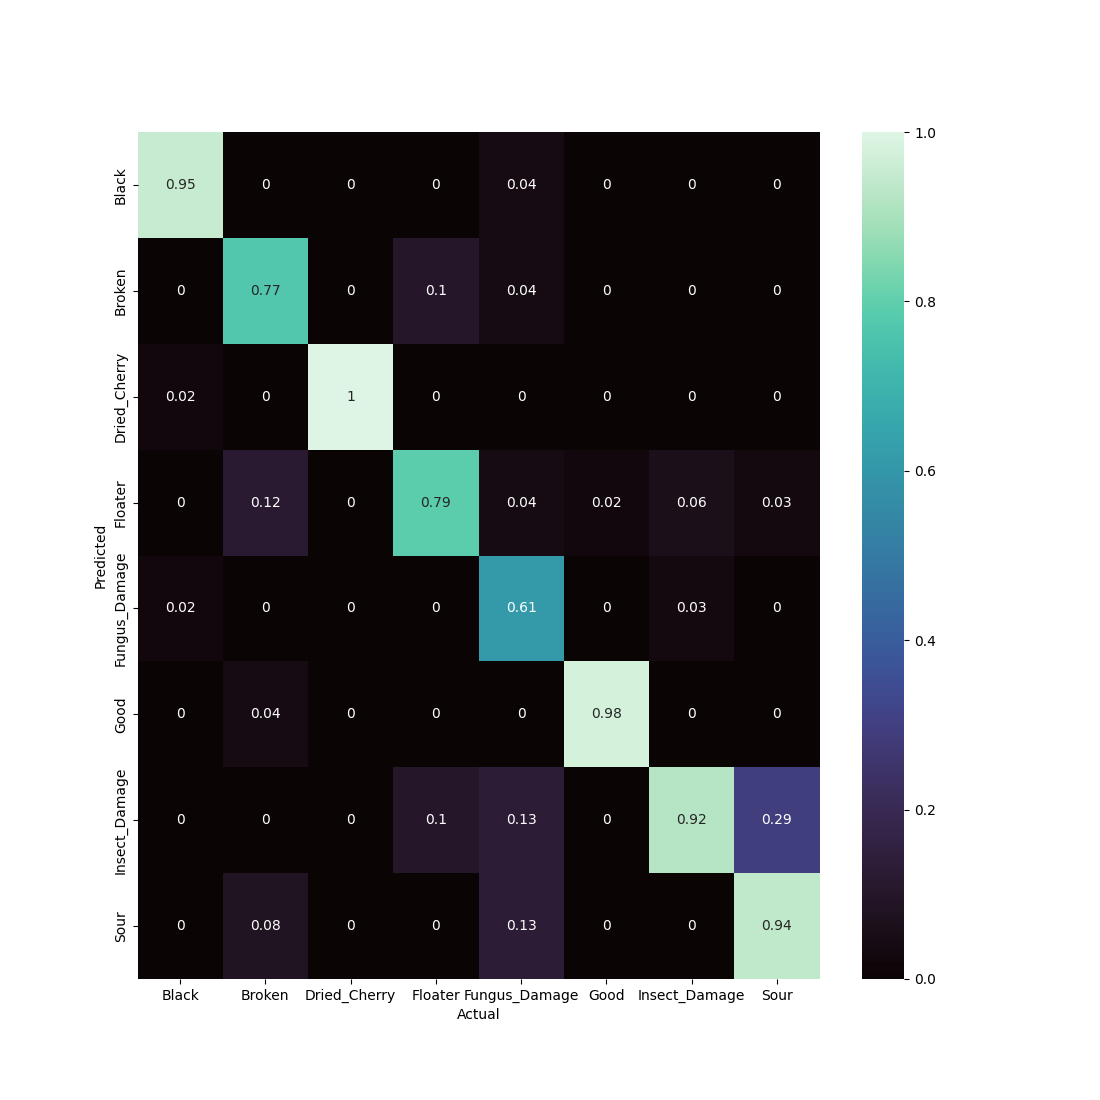
\includegraphics[width=\textwidth]{ch6/norm_effnet_confmatrix.png} % replace with image path
    \caption{Normalized Confusion Matrix for EfficientNetV2S on Test Dataset}
    \label{fig:effnetv2s_conf_matrix}
\end{figure}

EfficientNetV2 maintained competitive recognition for Black (95\%), Dried Cherry (100\%), and Good (98\%), but defect categories performed poorly. Fungus Damage was the weakest across all models (61\%), with extensive misclassification into Insect Damage and Sour. Broken scored only 77\%, spilling into Floater and Sour. Sour beans had 94\% recognition but with 29\% misclassified as Insect Damage. While good at separating distinct classes, this model struggles most with subtle defect patterns.

\subsection{YOLOv8}

\begin{figure}[H]
    \centering
    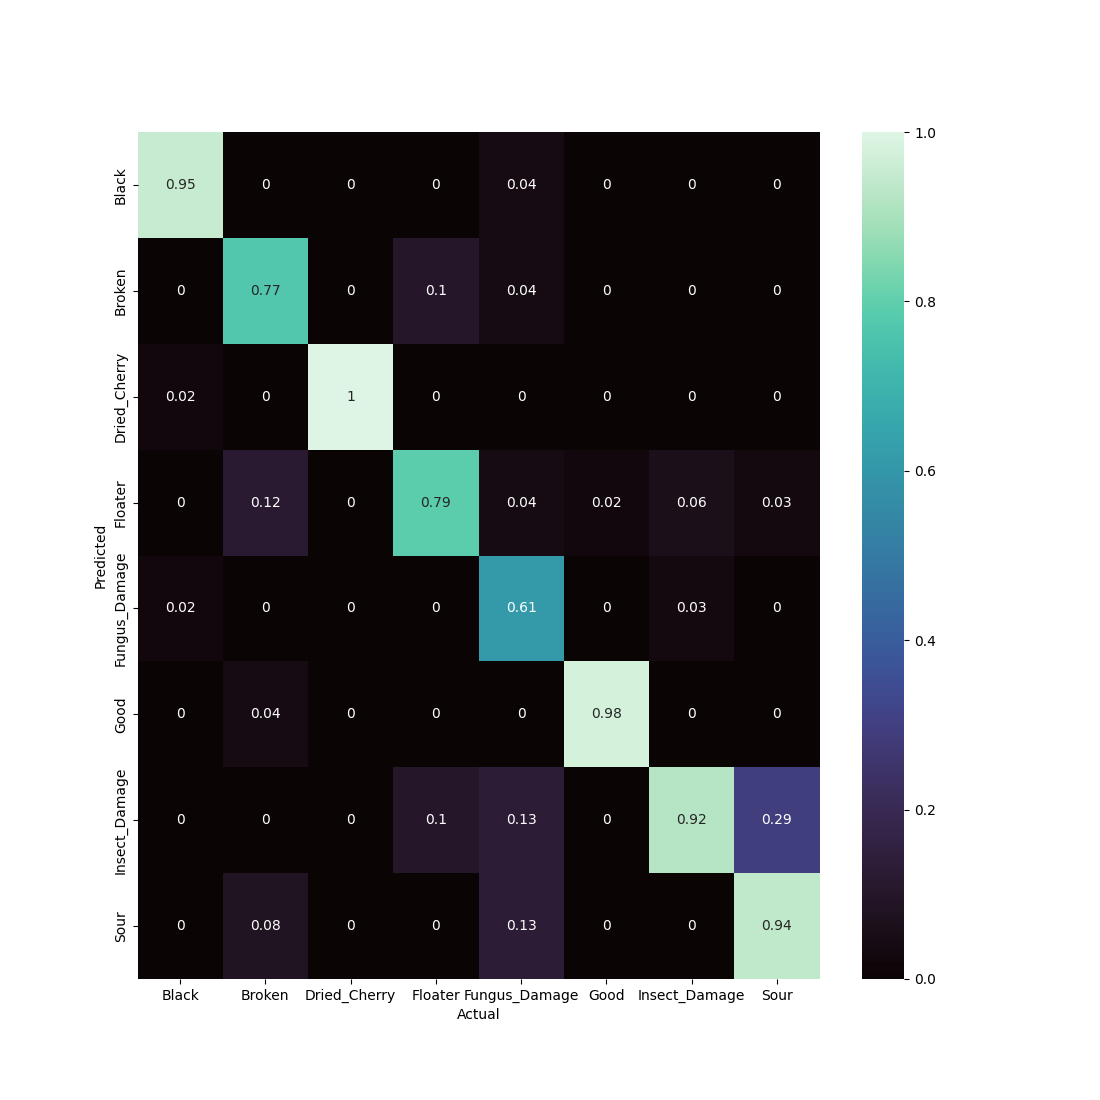
\includegraphics[width=\textwidth]{ch6/norm_v8_confmatrix.png} % replace with image path
    \caption{Normalized Confusion Matrix for YOLOv8 on Test Dataset}
    \label{fig:yolov8_conf_matrix}
\end{figure}

YOLOv8 achieved strong recognition for Black (98\%), Dried Cherry (100\%), Good (99\%), and Sour (100\%). However, it struggled with Fungus Damage (61\%), where a large share of samples were confused with Broken and Insect Damage. Broken was moderately accurate (85\%) but often mistaken as Floater. Insect Damage was fairly strong (94\%) yet confused back into Fungus Damage. The model excels at highly distinctive classes but struggles with visually similar defects.

\subsection{YOLOv11-cls}

\begin{figure}[H]
    \centering
    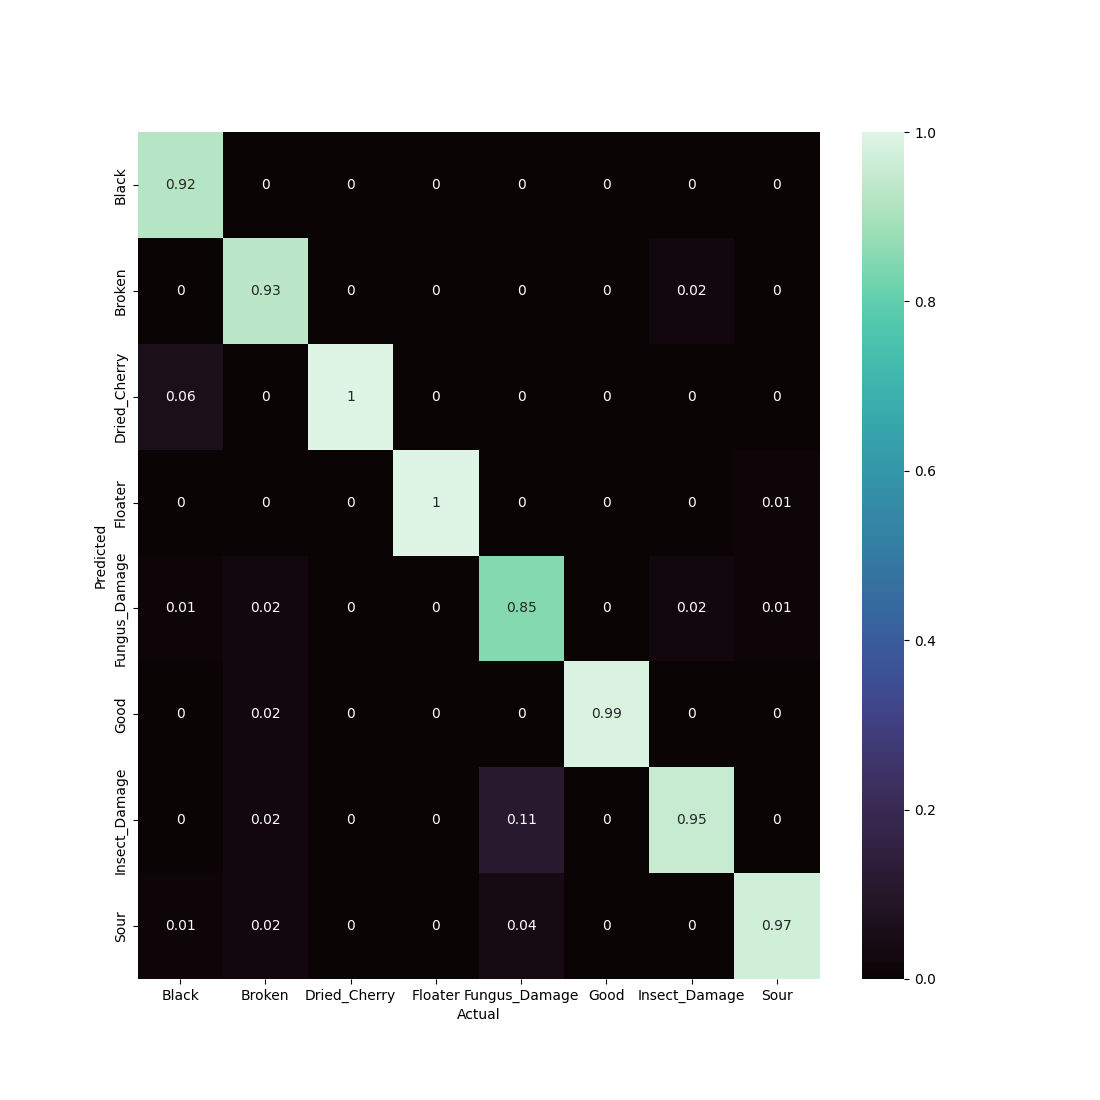
\includegraphics[width=\textwidth]{ch6/norm_v11_confmatrix.png} % replace with image path
    \caption{Normalized Confusion Matrix for YOLOv11 on Test Dataset}
    \label{fig:yolov11_conf_matrix}
\end{figure}

YOLOv11 improved class balance compared to YOLOv8, with near-perfect results in Dried Cherry, Floater, and Good (all 99–100\%). Broken rose to 93\%, reducing cross-class errors. Fungus Damage remained difficult at 85\%, misclassified into Broken, Insect Damage, and Sour. Insect Damage achieved 95\% but still leaked into Fungus Damage. This model demonstrates more stability in defect-prone categories while maintaining high precision in separable classes.

\subsection{YOLOv12-cls}

\begin{figure}[H]
    \centering
    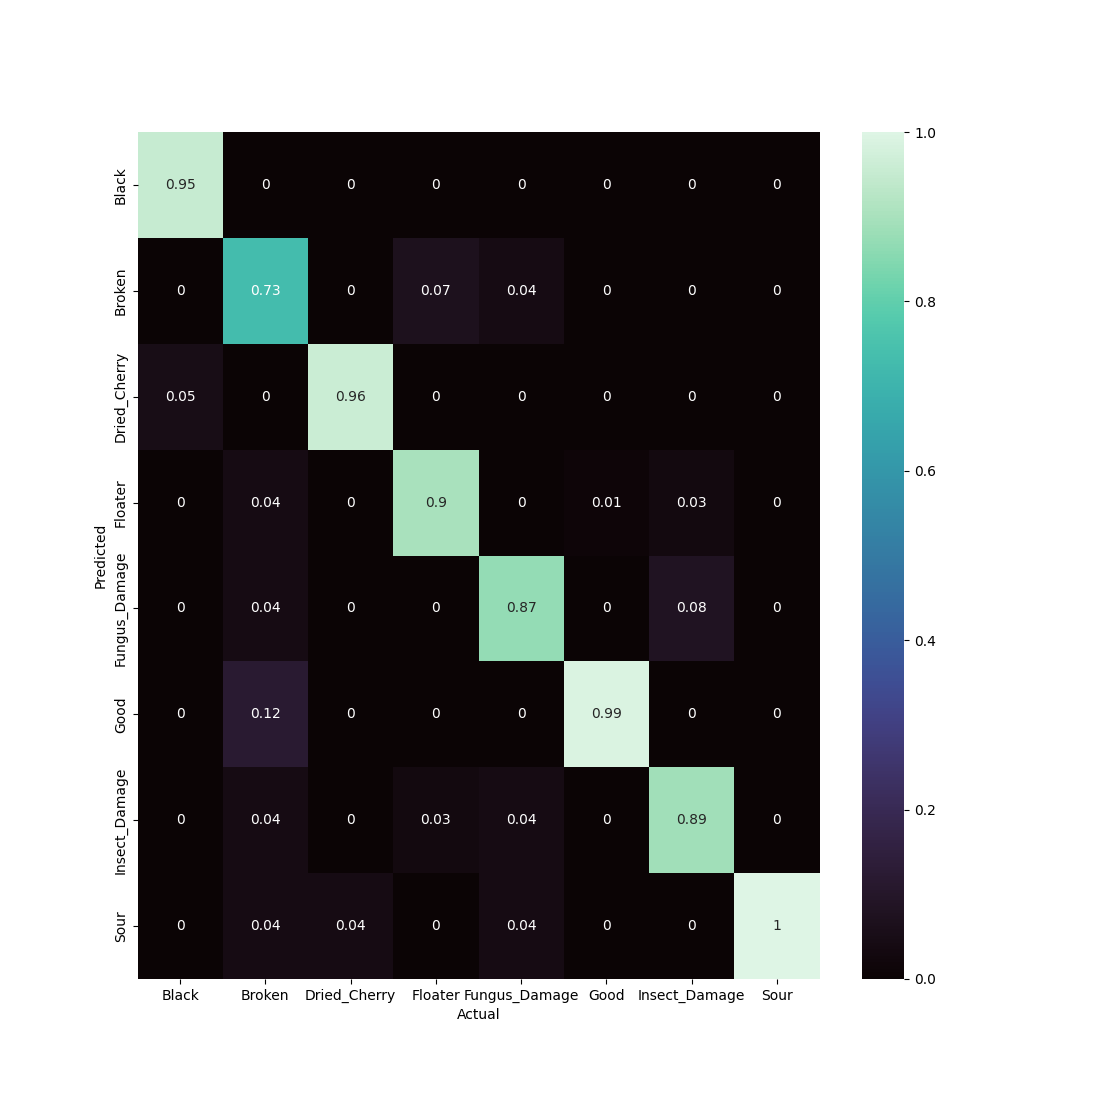
\includegraphics[width=\textwidth]{ch6/norm_v12_confmatrix.png} % replace with image path
    \caption{Normalized Confusion Matrix for YOLOv12 on Test Dataset}
    \label{fig:yolov12_conf_matrix}
\end{figure}

YOLOv12 presented mixed performance: Dried Cherry (96\%), Good (99\%), and Sour (100\%) stayed strong, but Broken collapsed to 73\%, with heavy confusion into Floater and Fungus Damage. Fungus Damage was moderate (87\%) but overlapped with Insect Damage (8\%). Insect Damage itself dropped to 89\%, reflecting this reciprocal confusion. Compared to YOLOv11, YOLOv12 was less stable on defect-heavy categories, showing variability despite strong results in clearer classes.

\subsection{Vision Transformer (ViT)}

\begin{figure}[H]
    \centering
    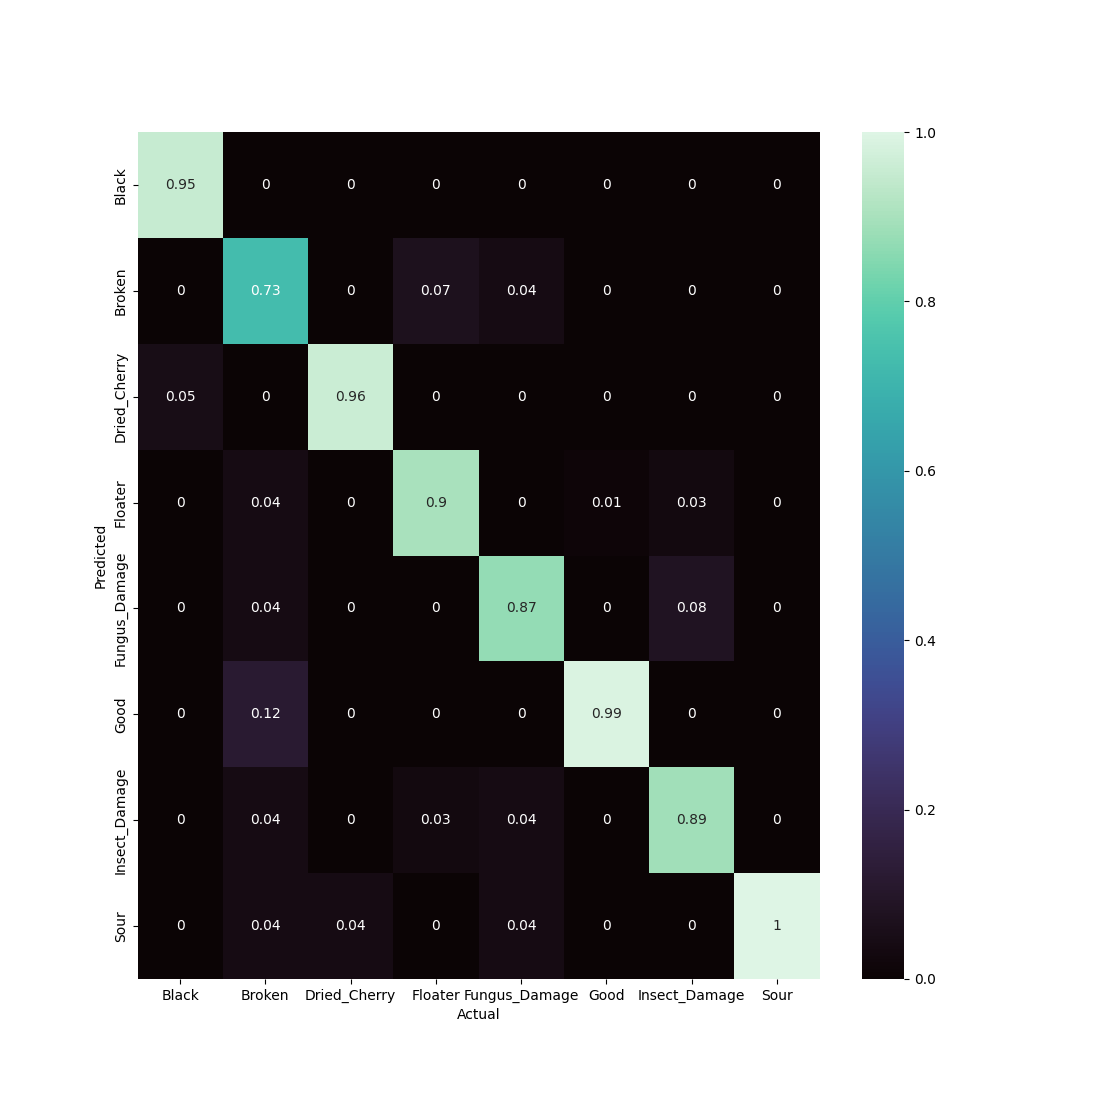
\includegraphics[width=\textwidth]{ch6/norm_v12_confmatrix.png} % replace with image path
    \caption{Normalized Confusion Matrix for ViT on Test Dataset}
    \label{fig:vit_conf_matrix}
\end{figure}

The ViT model delivered the most consistent results overall. Black and Dried Cherry were perfectly classified (100\%), while Good, Insect Damage, and Sour exceeded 97\%. Broken reached 92\%, with minor leakage into Floater and Fungus Damage. Floater held 93\% accuracy, though with 7\% misclassified as Broken. Fungus Damage was stronger than in other models (87\%) but still overlapped with Insect Damage (9\%). ViT demonstrates the best balance, minimizing confusion between defects while maintaining near-perfect performance in distinct classes.

\begin{table}[ht]
	\centering
	\caption{Model Performance Comparison}
	\label{tab:model_performance}
	\begin{tabular}{l c c c c}
	\toprule
	\textbf{Model} & \textbf{Precision (\%)} & \textbf{Recall (\%)} & \textbf{F1-Score (\%)} & \textbf{Accuracy (\%)} \\
	\midrule
	EfficientNetV2 & 87.90 & 87.08 & 87.08 & 98.02 \\
	YOLOv8        & 91.14 & 90.41 & 90.55 & 98.65 \\
	YOLOv11       & 92.97 & 93.71 & 93.19 & 98.90 \\
	YOLOv12       & 91.97 & 91.20 & 91.47 & 98.64 \\
	\textbf{ViT}  & \textbf{95.85} & \textbf{95.76} & \textbf{95.77} & \textbf{99.35} \\
	\bottomrule
	\end{tabular}
\end{table}

Table \ref{tab:model_performance} shows that EfficientNetV2 had the weakest performance, with the lowest precision, recall, F1-score, and accuracy. The YOLO models improved on these results, with YOLOv11 performing slightly better than YOLOv8 and YOLOv12. Among all, ViT achieved the highest scores across all metrics, showing the best ability to classify the test dataset with minimal errors. Overall, performance increases from EfficientNetV2 to YOLO, with ViT giving the most reliable results.

\section{Actual Performance of Classification Models in the System}

Among the 5 models, YOLOv12 and ViT achieved the highest performance. Thus, these two models were tested and deployed on the actual system. To measure the performance of the two models, two types of tests were conducted. The first test was conducted to measure the models’ performances on classifying different defect types, and the other test was dedicated to measuring the models’ performances when classifying Good and Defective beans . The first test set was composed of 30 beans per defect and 150 good beans, with a total of 360 beans. For each trial, the testing was divided into 8, corresponding to each classification. True Positives (TP) are the number of samples from a defect type that were correctly classified as that defect. False Negatives (FN) are the number of samples from a defect type that were misclassified as something else. Per-class accuracy was computed for each trial and the average accuracy across all trials. On the other hand, the second test was composed of 100 beans per trial, wherein each trial had a varying distribution of good and defective beans. In this test, TP is the number of good beans classified as good, TN is the number of defective beans classified as defects, FP is the number of defective beans misclassified as good, and FN is the number of good beans misclassified as defects. 

\begin{figure}[H]
    \centering
    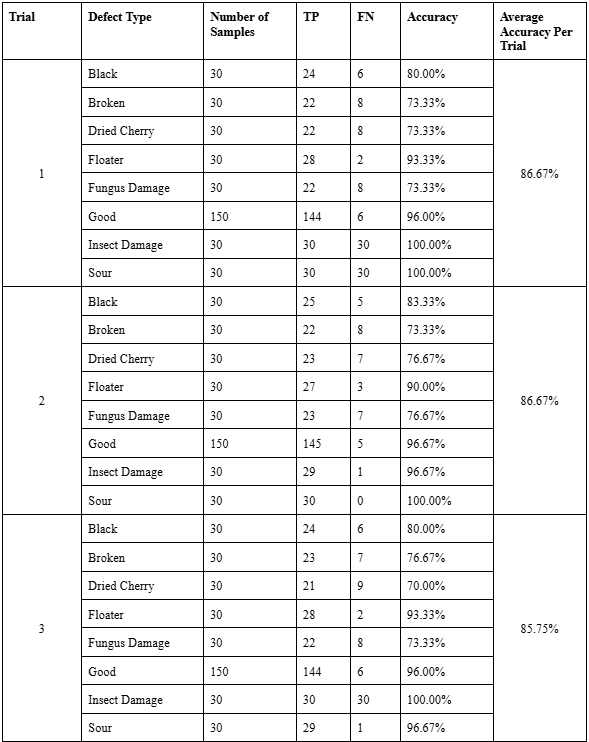
\includegraphics[width=0.8\textwidth]{ch6/Actual_Performance_of_YOLOv12_p1.png}
    \label{fig:actual_performance_v12}
\end{figure}

\begin{figure}[H]
    \centering
    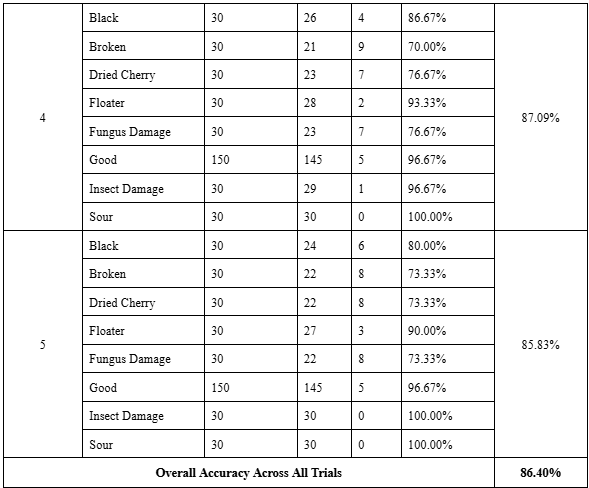
\includegraphics[width=0.8\textwidth]{ch6/Actual_Performance_of_YOLOv12_p2.png}
    \caption{Actual Performance of YOLOv12 in the System (Per-Classification)}
    \label{fig:actual_performance_v12}
\end{figure}
Table \ref{fig:actual_performance_v12} represents the actual performance of YOLOv12 when deployed into the system. Across five trials, the results showed that the model achieved promising accuracy in certain categories like Insect Damage and Sour, where an accuracy of 100\% in some trials were recorded. Most importantly, the model’s performance on Good beans classification was highly reliable achieving 96-97\% across the different trials. However, it was observed that the model struggled with other categories such as Black, Broken, Fungus Damage, and Dried Cherry, achieving an accuracy score of only around 70-80\%. The overall accuracy of YOLOv12 across all the trials was 86.4\%, which is already reliable especially for detecting Good vs Defective beans. 

\begin{figure}[H]
    \centering
    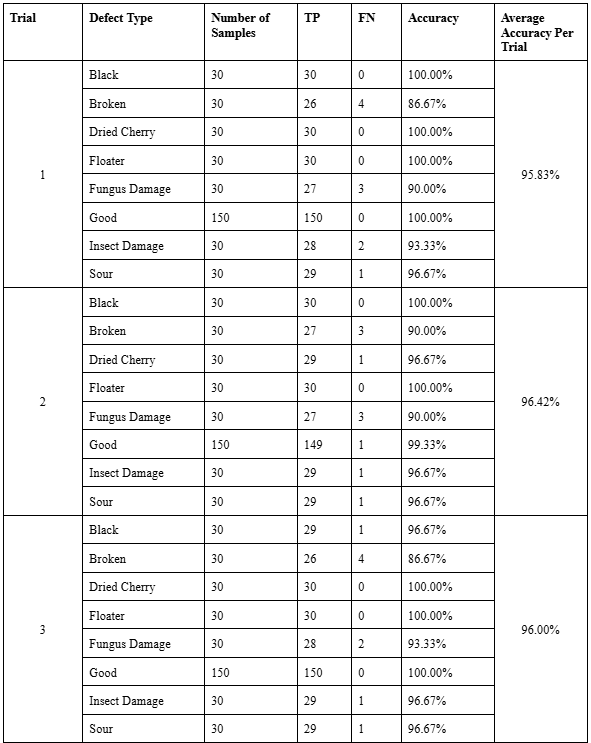
\includegraphics[width=0.8\textwidth]{ch6/Actual_Performance_of_ViT_p1.png}
    \label{fig:actual_performance_vit}
\end{figure}

\begin{figure}[H]
    \centering
    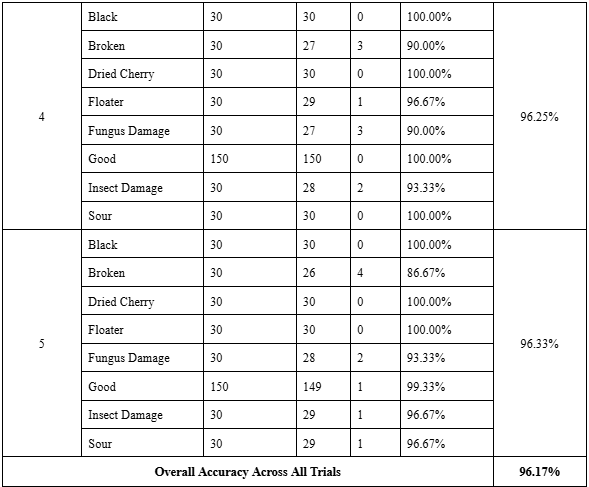
\includegraphics[width=0.8\textwidth]{ch6/Actual_Performance_of_ViT_p2.png}
    \caption{Actual Performance of ViT in the System (Per-Classification)}
    \label{fig:actual_performance_vit}
\end{figure}
In Table \ref{fig:actual_performance_vit}, the performance of the Vision Transformer (ViT) model across all five trials were presented. The recorded data shows that ViT was more consistent than the YOLOv12, achieving very high accuracy scores in classifying Black, Dried Cherry, Floater, Sour, and Good beans. It was observed that the model even achieved perfect accuracies on these classifications on some trials. On the other hand, the model’s performance on classifying Broken beans was slightly lower but still reliable, achieving an accuracy between 86-90%. Across all five trials, the overall accuracy of the model was around 96%, which is a significant improvement from YOLOv12. This demonstrates that ViT not only generalized well across multiple defect categories, but also maintained consistency during repeated testing.

\begin{table}[ht]
	\centering
	\small
	\caption{Actual Performance of YOLOv12 in the System (Good vs. Defect)}
	\begin{tabularx}{\linewidth}{@{}>{\raggedright}X c c c c c@{}}
	\toprule
	\textbf{Test Condition} & \textbf{TP} & \textbf{TN} & \textbf{FP} & \textbf{FN} & \textbf{Accuracy (\%)} \\
	\midrule
	100\% Good Beans & 89 & 0 & 0 & 11 & 89 \\
	75\% Good, 25\% Defective & 71 & 24 & 1 & 4 & 95 \\
	50\% Good, 50\% Defective & 49 & 49 & 1 & 1 & 98 \\
	25\% Good, 75\% Defective & 23 & 72 & 3 & 2 & 95 \\
	100\% Defective Beans & 0 & 97 & 3 & 0 & 97 \\
	\bottomrule
	\textbf{Average Accuracy} & & & & & \textbf{94.8} \\
	\end{tabularx}
	\label{tab:yolov12_good_defective}
\end{table}

Table \ref{tab:yolov12_good_defective} presents the performance of YOLOv12 on classifying good and defective beans under varying test conditions. Compared to the model’s per-classification performance, the results demonstrated higher accuracy  when classifying good and defective beans. The model achieved an average accuracy of  94.8\% across all trials with varying test conditions. These findings indicate that YOLOv12 can be a reliable model when simply sorting between the two classifications.

\begin{table}[ht]
	\centering
	\small
	\caption{Actual Performance of ViT in the System (Good vs. Defect)}
	\begin{tabularx}{\linewidth}{@{}>{\raggedright}X c c c c c@{}}
	\toprule
	\textbf{Test Condition} & \textbf{TP} & \textbf{TN} & \textbf{FP} & \textbf{FN} & \textbf{Accuracy (\%)} \\
	\midrule
	100\% Good Beans & 100 & 0 & 0 & 0 & 100 \\
	75\% Good, 25\% Defective & 72 & 24 & 1 & 3 & 96 \\
	50\% Good, 50\% Defective & 48 & 50 & 0 & 2 & 98 \\
	25\% Good, 75\% Defective & 23 & 75 & 0 & 2 & 98 \\
	100\% Defective Beans & 0 & 98 & 2 & 0 & 98 \\
	\bottomrule
	\textbf{Average Accuracy} & & & & & \textbf{98} \\
	\end{tabularx}
	\label{tab:vit_good_defective}
\end{table}

On the other hand, Table \ref{tab:vit_good_defective} presents the data on the performance of ViT model under varying proportions of good and defective beans. The model achieved an average accuracy of 98\% across all five trials, which was similar to its per-classification accuracy. Thus, showing reliability and consistency on its accuracy on both per-classification testing (defect types) and binary testing (good and defect).

\newpage
\section{Sorting Speed}

\label{sec:sorting_speed}
\begin{table}[ht]
	\centering
	\small
	\caption{Sorting Speed Test Conditions}
	\label{tab:sorting_speed_test}
	\begin{tabularx}{\linewidth}{@{}>{\raggedright}X c c c@{}}
	\toprule
	\textbf{Test Condition} & \textbf{Conveyor (RPM)} & \textbf{Inspection (RPM)} & \textbf{Sorting (Beans/min)} \\
	\midrule
	100\% Good Beans & 175 & 343 & 22 \\
	80\% Good, 20\% Defective & 175 & 343 & 22 \\
	70\% Good, 30\% Defective & 175 & 343 & 21 \\
	50\% Good, 50\% Defective & 175 & 343 & 24 \\
	100\% Defective Beans & 175 & 343 & 22 \\
	\bottomrule
	\end{tabularx}
\end{table}
Table \ref{tab:sorting_speed_test} presents the prototype system's sorting speed performance under different test conditions. The conveyor table speed and inspection tray motor speed is constant at 175 RPM and 343 RPM, respectively, to ensure consistency in all trials. The sorting speed, expressed in beans per minute, indicates the system's capacity to recognize and process coffee beans. The outcomes indicate that the system maintained a steady average sorting rate of 22 beans per minute in most conditions, such as 100\% good beans, 80:20, and 100\% defective beans. The minimal drop to 21 beans per minute under the 70\% good and 30\% defective condition could be due to the long wait time for the beans to fall onto the inspection tray. On the other hand, the peak sorting rate of 24 beans per minute under the 50:50 condition indicates that the system's classification and actuations were synchronized. Overall, the prototype proves to have stable and consistent sorting throughput. The results confirm that the system can work at a steady speed appropriate for small-scale processing operations without degradation in performance by the number of defective beans.

\begin{figure}[H]
    \centering
    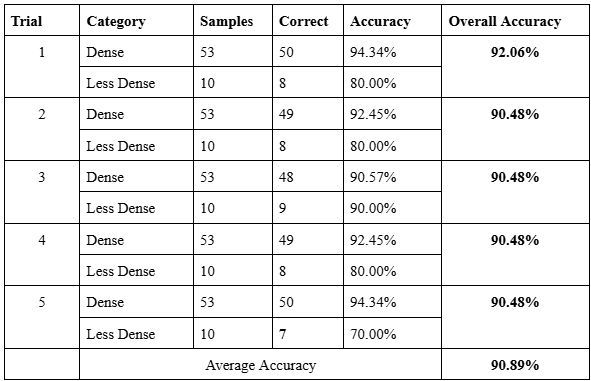
\includegraphics[width=0.8\textwidth]{ch6/Actual_Density_Sorting_Performance.png}
    \caption{Actual Density Sorting Performance}
    \label{fig:actual_density_sorting_performance}
\end{figure}

Table \ref{fig:actual_density_sorting_performance} presents the results of five trials evaluating the density sorting mechanism. The system consistently classified dense beans with high accuracy, ranging from 90.57\% to 94.34\%, showing that the sorter was generally reliable in distinguishing beans with higher density. In contrast, the classification of less dense beans fluctuated more significantly, with accuracies between 70.00\% and 90.00\%, indicating that this category posed greater difficulty for the system. Overall accuracies across the trials remained relatively stable, ranging from 90.48\% to 92.06\% with an average accuracy of 90.89\%, which demonstrates consistent sorting performance but also highlights that occasional misclassifications prevented the system from reaching perfect accuracy. These findings suggest that while the sorter is effective in identifying dense beans, improvements may be needed in refining the sensitivity of the system to reliably classify less dense beans.

